\newpage
\section{第 03 周}

\subsection{第 8 课 | 分治、回溯}

\subsubsection{脑图}

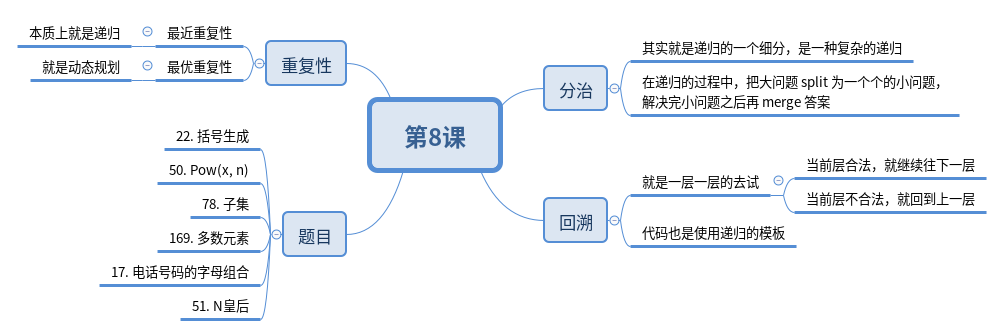
\includegraphics[width=170mm,height=80mm]{images/camp/第8课.png}

\subsubsection{题目}

\begin{itemize}
  \item \hyperref[leetcode:22]{22. 括号生成}
  \item \hyperref[leetcode:50]{50. Pow(x, n)}
  \item \hyperref[leetcode:78]{78. 子集}
  \item \hyperref[leetcode:169]{169. 多数元素}
  \item \hyperref[leetcode:17]{17. 电话号码的字母组合}
  \item \hyperref[leetcode:51]{51. N皇后}
\end{itemize}

\subsection{第 9 课 | DFS 和 BFS}

\subsubsection{脑图}

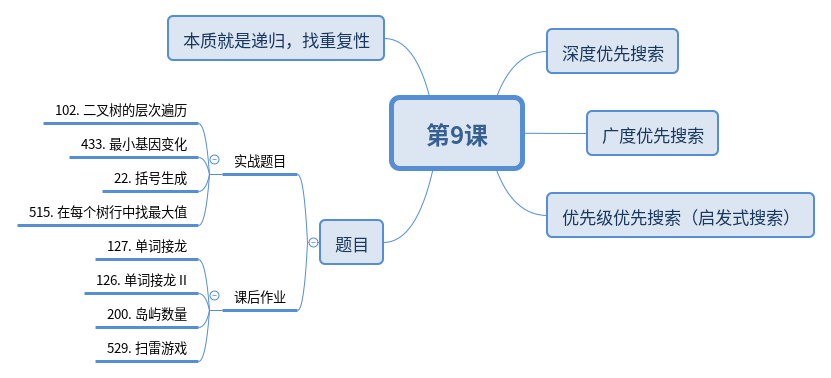
\includegraphics[width=170mm,height=80mm]{images/camp/第9课.png}

\subsubsection{题目}

\paragraph{实战题目}

\begin{itemize}
  \item \hyperref[leetcode:102]{102. 二叉树的层次遍历}
  \item \hyperref[leetcode:433]{433. 最小基因变化}
  \item \hyperref[leetcode:22]{22. 括号生成}
  \item \hyperref[leetcode:515]{515. 在每个树行中找最大值}
\end{itemize}

\paragraph{课后作业}

\begin{itemize}
  \item \hyperref[leetcode:127]{127. 单词接龙}
  \item \hyperref[leetcode:126]{126. 单词接龙 II}
  \item \hyperref[leetcode:200]{200. 岛屿数量}
  \item \hyperref[leetcode:529]{529. 扫雷游戏}
\end{itemize}

\subsection{第 10 课 | 贪心算法}

\subsubsection{脑图}

\subsubsection{题目}

\subsection{第 11 课 | 二分查找}

\subsubsection{脑图}

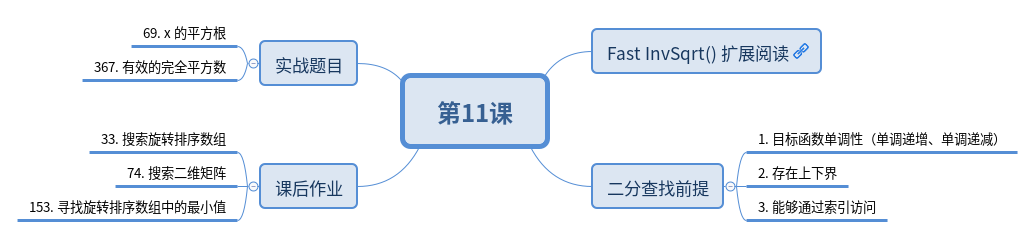
\includegraphics[width=170mm,height=80mm]{images/第11课.png}

\subsubsection{题目}

\paragraph{实战题目}

\begin{itemize}
  \item \hyperref[leetcode:69]{69. x 的平方根}
  \item \hyperref[leetcode:367]{367. 有效的完全平方数}
\end{itemize}

\paragraph{课后作业}

\begin{itemize}
  \item \hyperref[leetcode:33]{33. 搜索旋转排序数组}
  \item \hyperref[leetcode:74]{74. 搜索二维矩阵}
  \item \hyperref[leetcode:153]{153. 寻找旋转排序数组中的最小值}
  \item 使用二分查找,寻找一个半有序数组 [4, 5, 6, 7, 0, 1, 2] 中间无序的地方
    说明:同学们可以将自己的思路、代码写在第 3 周的学习总结中
\end{itemize}


\subsection{学习总结}

这周学习了分治,回溯,深度优先搜索,广度优先搜索,
贪心算法,二分查找。

分治其实就是递归的一个细分,是一种复杂的递归。在
递归的过程中,把大问题 split 为一个个的小问题,
解决完小问题之后再 merge 答案。

回溯就是在递归的过程中,如果不合法的话,就回到上一层。

搜索分为深度优先搜索,广度优先搜索,优先级优先搜索。
我们需要熟练掌握深度优先搜索和广度优先搜索。

对于深度优先搜索和广度优先搜索我有一个思考,深度优先搜索
的非递归版本是用一个栈来保存中间节点,而广度优先搜索是用
队列来保存中间节点,那要是我用一个随机的容器来保存节点,
那是不是就能够得到一个随机搜索,但是最终也是一样可以遍历
到所有的节点。

贪心法:局部最优,同时也能够得到全局最优。\\
动态规划:局部最优无法得到全局最优时,就需要用动态规划。

二分查找前提:目标函数单调性。存在上下界。能够通过索引访问。
